\section{Solution of the problem of elasticity theory \parencite{ref5} }\label{theory}
In this section, we discuss elastic theoretical equations help to establish the problem.

\begin{itemize}
\item 3 equilibrium equations
    \begin{equation}
        \begin{split}
        \frac{{\partial {\sigma _x}}}{{\partial x}} + \frac{{\partial {\tau _{yx}}}}{{\partial y}} + \frac{{\partial {\tau _{zx}}}}{{\partial z}} + X = 0\\
        \frac{{\partial {\tau _{xy}}}}{{\partial x}} + \frac{{\partial {\sigma _y}}}{{\partial y}} + \frac{{\partial {\tau _{zy}}}}{{\partial z}} + Y = 0\\
        \frac{{\partial {t_{xz}}}}{{\partial x}} + \frac{{\partial {\tau _{yz}}}}{{\partial y}} + \frac{{\partial {\sigma _z}}}{{\partial z}} + Z = 0
        \end{split}
    \end{equation}
\item 6 deformation equations
\begin{list}{+}{}
    \item By Cauchy:
        \begin{equation}
    \begin{split}
        {{\varepsilon _x} = \frac{{\partial u}}{{\partial x}}; \qquad}&{{y_{xy}} = \frac{{\partial u}}{{\partial y}} + \frac{{\partial v}}{{\partial x}}}\\
        {{\varepsilon _y} = \frac{{\partial v}}{{\partial y}}; \qquad}&{{y_{yz}} = \frac{{\partial v}}{{\partial z}} + \frac{{\partial w}}{{\partial y}}}\\
        {{\varepsilon _z} = \frac{{\partial w}}{{\partial z}}; \qquad}&{{y_{zx}} = \frac{{\partial w}}{{\partial x}} + \frac{{\partial u}}{{\partial z}}}
    \end{split}
    \end{equation}
    \item By Saint-Venant:
    \begin{equation}
        \begin{gathered}
\frac{{{\partial ^2}{\gamma _{xy}}}}{{\partial x\partial y}} = \frac{{{\partial ^2}{\varepsilon _x}}}{{\partial {y^2}}} + \frac{{{\partial ^2}{\varepsilon _y}}}{{\partial {x^2}}}\\
\frac{{{\partial ^2}{y_{yz}}}}{{\partial y\partial z}} = \frac{{{\partial ^2}{\varepsilon _y}}}{{\partial {z^2}}} + \frac{{{\partial ^2}{\varepsilon _z}}}{{\partial {y^2}}}\\
\frac{{{\partial ^2}{y_{zx}}}}{{\partial z\partial x}} = \frac{{{\partial ^2}{\varepsilon _z}}}{{\partial {x^2}}} + \frac{{{\partial ^2}{\varepsilon _x}}}{{\partial {z^2}}}\\
2\frac{{{\partial ^2}{\varepsilon _x}}}{{\partial y\partial z}} = \frac{\partial }{{\partial x}}\left( {\frac{{ - \partial {y_{yz}}}}{{\partial x}} + \frac{{\partial {\gamma _{zx}}}}{{\partial y}} + \frac{{\partial {\gamma _{xy}}}}{{\partial z}}} \right)\\
2\frac{{{\partial ^2}{\varepsilon _y}}}{{\partial z\partial x}} = \frac{\partial }{{\partial y}}\left( {\frac{{\partial {y_{yz}}}}{{\partial x}} - \frac{{\partial {y_{zx}}}}{{\partial y}} + \frac{{\partial {y_{xy}}}}{{\partial z}}} \right)\\
2\frac{{{\partial ^2}{\varepsilon _z}}}{{\partial x\partial y}} = \frac{\partial }{{\partial z}}\left( {\frac{{\partial {y_{yz}}}}{{\partial x}} + \frac{{\partial {\gamma _{zx}}}}{{\partial y}} - \frac{{\partial {y_{xy}}}}{{\partial z}}} \right)
\end{gathered}
    \end{equation}
\end{list}
\item Stress-Strain Relationship \parencite{ref4}
\begin{list}{+}{}
\item Stress–strain relationship for isotropic material :

 Robert Hooke was the first one to propose the linear uniaxial stress–strain relation, which states that the stress is proportional to strain. Later, the general relation between the six components of strains and stresses called the generalized Hooke’s law was developed. The generalized Hooke’s law states that each component of stress is a linear combination of strains.

 The stress–strain relationship can be written as: 
 \begin{equation}
    \begin{gathered}
        {\sigma _x} = 2G\left( {{\varepsilon _x} + \frac{{3\mu }}{{1 - 2\mu }}{\varepsilon _{tb}}} \right)\\
        {\sigma _y} = 2G\left( {{\varepsilon _y} + \frac{{3\mu }}{{1 - 2\mu }}{\varepsilon _{tb}}} \right)\\
        {\sigma _z} = 2G\left( {{\varepsilon _z} + \frac{{3\mu }}{{1 - 2\mu }}{\varepsilon _{tb}}} \right)\\
        {\tau _{xv}} = G{Y_{xv}},{\tau _{vz}} = G{Y_{vz}},{\tau _{zx}} = G{Y_{zx}}
\end{gathered}
 \end{equation}

Or we can write it another way:
\begin{equation}
\begin{gathered}
{\varepsilon _x} = \frac{1}{E}\left[ {{\sigma _x} - \mu \left( {{\sigma _y} + {\sigma _z}} \right)} \right]\\
{\varepsilon _y} = \frac{1}{E}\left[ {{\sigma _y} - \mu \left( {{\sigma _x} + {\sigma _z}} \right)} \right]\\
{\varepsilon _z} = \frac{1}{E}\left[ {{\sigma _z} - \mu \left( {{\sigma _x} + {\sigma _y}} \right)} \right]\\
{Y_{xy}} = \frac{{{\tau _{xy}}}}{G};{y_{yz}} = \frac{{{\tau _{yz}}}}{G};{y_{zx}} = \frac{{{\tau _{zx}}}}{G}
\end{gathered}
\end{equation}

\item Stress–strain relationship for Material Nonlinearity:

In non-linear materials, their relationship is non-linear, which we will discuss in the next chapter
\begin{figure}[H]
    \centering
    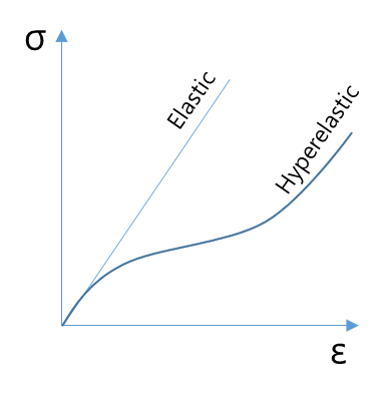
\includegraphics[scale=1]{Figures/Hyperelastic.png}
    \decoRule   
    \caption{ Difference between linear and non-linear material in stress–strain relationship}
    \label{fig:Electron}
\end{figure}
\end{list}
\end{itemize}
%------------------------------------------------------------------------------------------------